\documentclass[tikz,border=3.14mm]{standalone}
\usetikzlibrary{patterns,decorations.pathmorphing,positioning}
\begin{document}
	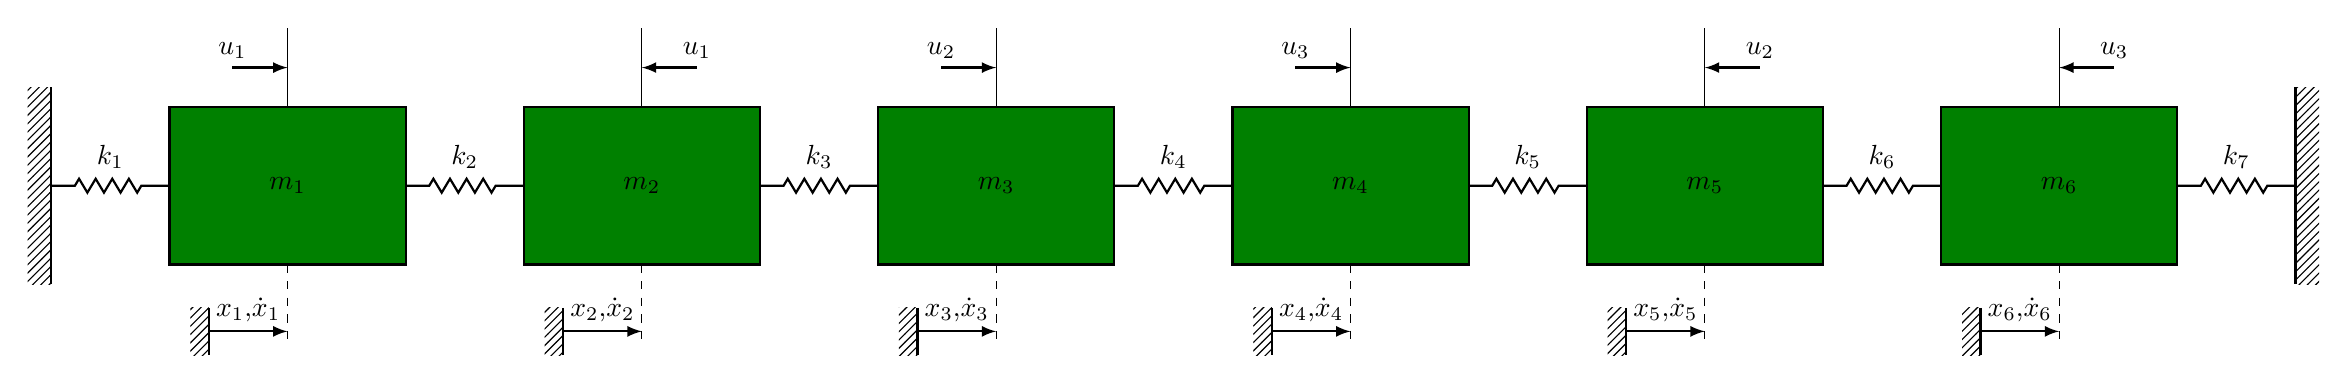
\begin{tikzpicture}[every node/.style={outer sep=0pt},thick,
		mass/.style={draw,thick},
		spring/.style={thick,decorate,decoration={zigzag,pre length=0.3cm,post
				length=0.3cm,segment length=6}},
		ground_1/.style={fill,pattern=north east lines,draw=none,minimum
			width=0.75cm,minimum height=0.3cm},
		ground_2/.style={fill,pattern=north east lines,draw=none,minimum
			width=0.75cm,minimum height=0.3cm},
		dampic/.pic={\fill[white] (-0.1,-0.3) rectangle (0.3,0.3);
			%\draw (-0.3,0.3) -| (0.3,-0.3) -- (-0.3,-0.3);
			\draw[line width=1mm] (-0.1,-0.3) -- (-0.1,0.3);}]
		
		\node[mass,minimum width=3.0cm,minimum height=2cm,fill=green!50!black] (m1) {$m_1$};
		\node[mass,minimum width=3.0cm,minimum height=2cm,fill=green!50!black,right=1.5cm of
		m1] (m2) {$m_2$};
		\node[mass,minimum width=3.0cm,minimum height=2cm,fill=green!50!black,right=1.5cm of
		m2] (m3) {$m_3$};
		\node[mass,minimum width=3.0cm,minimum height=2cm,fill=green!50!black,right=1.5cm of
		m3] (m4) {$m_4$};
		\node[mass,minimum width=3.0cm,minimum height=2cm,fill=green!50!black,right=1.5cm of
		m4] (m5) {$m_5$};
		\node[mass,minimum width=3.0cm,minimum height=2cm,fill=green!50!black,right=1.5cm of
		m5] (m6) {$m_6$};
		
		
		\node[left=1.5cm of m1,ground_1,minimum width=3mm,minimum height=2.5cm] (g1){};
		\draw (g1.north east) -- (g1.south east);
		
		\draw[spring] ([yshift=0mm]g1.east) coordinate(aux)
		-- (m1.west) node[midway,above=1mm]{$k_1$};
		\draw[spring]  (m1.east) -- (m2.west) node[midway,above=1mm]{$k_2$};
		\draw[spring]  (m2.east) -- (m3.west) node[midway,above=1mm]{$k_3$};
		\draw[spring]  (m3.east) -- (m4.west) node[midway,above=1mm]{$k_4$};
		\draw[spring]  (m4.east) -- (m5.west) node[midway,above=1mm]{$k_5$};
		\draw[spring]  (m5.east) -- (m6.west) node[midway,above=1mm]{$k_6$};
		
		\node[right=1.5cm of m6,ground_2,minimum width=3mm,minimum height=2.5cm] (g2){};
		\draw (g2.north west) -- (g2.south west);

		\draw[spring]  (m6.east) -- ([yshift=0mm]g2.west) coordinate(aux) node[midway,above=1mm]{$k_7$};

		\foreach \X in {1,2,3,4,5,6}  
		{	
			%\draw[thin] (m\X.north) -- ++ (0,1) coordinate[midway](aux\X);
			%\draw[latex-] (aux\X) -- ++ (-0.5,0) 	node[above]{$F_\X$}; 
			\draw[thin,dashed] (m\X.south) -- ++ (0,-1) 	coordinate[pos=0.85](aux'\X);
			\draw[latex-] (aux'\X) -- ++ (-1,0) node[midway,above]{$x_\X$,$\dot{x}_\X$}
			node[left,ground_1,minimum height=6mm,minimum width=1mm] (g'\X){};
			\draw[thick] (g'\X.north east) -- (g'\X.south east);
		}
		
		\draw[thin] (m1.north) -- ++ (0,1) coordinate[midway](aux1);
		\draw[latex-] (aux1) -- ++ (-0.7,0) 	node[above]{$u_1$}; 

		\draw[thin] (m2.north) -- ++ (0,1) coordinate[midway](aux2);
		\draw[latex-] (aux2) -- ++ (+0.7,0) 	node[above]{$u_1$}; 				
		
		\draw[thin] (m3.north) -- ++ (0,1) coordinate[midway](aux3);
		\draw[latex-] (aux3) -- ++ (-0.7,0) 	node[above]{$u_2$};
		
		\draw[thin] (m4.north) -- ++ (0,1) coordinate[midway](aux4);
		\draw[latex-] (aux4) -- ++ (-0.7,0) 	node[above]{$u_3$};
		
		\draw[thin] (m5.north) -- ++ (0,1) coordinate[midway](aux5);
		\draw[latex-] (aux5) -- ++ (+0.7,0) 	node[above]{$u_2$};
		
		\draw[thin] (m6.north) -- ++ (0,1) coordinate[midway](aux6);
		\draw[latex-] (aux6) -- ++ (+0.7,0) 	node[above]{$u_3$};
		
	\end{tikzpicture}
\end{document}